\documentclass[12pt]{article}

% Sets document language to English (some british conventions in
% hyphenation). Can also handle multilingual documents.
\usepackage[british]{babel}
\usepackage{csquotes}
\usepackage{pdflscape} 
\usepackage{geometry}
\usepackage{longtable}

% Uses the newer biblatex (with biber as backend) for citations and
% references. Can deal with non-ascii letters in author names.
\usepackage{biblatex}
\addbibresource{references.bib}

% Provides more maths support and the theorem environments.
\usepackage{amsmath}
\usepackage{amsthm}
\theoremstyle{plain}
\newtheorem{theorem}{Theorem}
\newtheorem{lemma}[theorem]{Lemma}
\theoremstyle{definition}
\newtheorem{definition}[theorem]{Definition}

% Font handling here is intended for LuaTeX or XeTeX engine.
% Sets the font. In this case a font similar to Times.
\usepackage{fontspec}
\setmainfont{TeX Gyre Termes}
\setmonofont{Source Code Pro}[Scale=MatchLowercase]
% Unicode math fonts
\usepackage{unicode-math}
\setmathfont{texgyretermes-math.otf}

% Some generally useful packages:
% Provides \includegraphics to insert images.
\usepackage{graphicx}
% Provides \url to insert url links.
\usepackage{url}
% Provides colour support.
\usepackage{xcolor}
% Provides tables that are aesthetically more pleasing.
\usepackage{booktabs}
% Provides more configurable itemised and enumerated lists.
\usepackage{enumitem}
% Provides environment for defining vector graphics drawings.
\usepackage{tikz}
% Provides environment for code listings.
\usepackage{listings}
\lstset{
  tabsize=2,
  breaklines=true,
  captionpos=b,
  extendedchars=true,
  numbers=left,
  basicstyle=\ttfamily,
  commentstyle=\color{red!70!black},
  keywordstyle=\color{green!70!black},
  numberstyle=\tiny\color{black!50},
  stringstyle=\ttfamily\color{blue!50!black},
  backgroundcolor=\color{yellow!10}
}
% Provides hyperlinks in the pdf. Not suitable for printed documents,
% but fine here.
\usepackage[pdfborder={0 0 0},colorlinks=true,allcolors={blue!40!black}]{hyperref}

% Load the style file (title page and declarations) for the document.
\usepackage[]{swanseaTitleUG}

% Paragraphs are typeset with a small skip between them.
\usepackage[parfill]{parskip} 

% User supplied information that appears on title page. Do edit these!
\title{ Project Specification and Planning}
\author{Katie Peacey}
\studentid{2214646}
\project{Shoulder Surfing Detector}

% Table of contents only lists 2 levels.
\setcounter{tocdepth}{2}

\begin{document}
\pagenumbering{roman}
\maketitle

% Build the table of contents page.
\tableofcontents

% These lists are optional, especially if they are empty.
\listoffigures
\listoftables
\clearpage

% Reset numeric page numbering from page 1
\pagenumbering{arabic}

\section{Introduction}
\label{sec:intro}

Shoulder surfing is the process of overlooking onto someone’s information without their permission, causing privacy and securing concerns \cite{eiband_understanding_2017}. This project looks into exploring current work and suggests ways in which shoulder surfing could be mitigated. Background research is explored to suggest tools that can be used to aid the project, and personas have been created to help understand the target audience.

\section{Motivation}
\label{sec:motivation} 

The exploration of ways to detect shoulder surfing attacks is continuous in academia, and the focus of this project is to suggest a way in which this can be done. The users experience will be central in this project, with multiple user studies being completed to understand their needs.
When working with other people's data, the General Data Protection Regulations (GDPR) \cite{noauthor_data_nodate} should always be adhered to. All data should be kept secure and only those who are authorised should have access \cite{noauthor_data_nodate}.

\subsection{Understanding Users}
An understanding on the type of users that would use the result of this project is important to address. The user will be a key factor throughout, and multiple user studies will be carried out to visualise their experiences.

\subsubsection{Personas}
This project allows for anyone who uses digital devices especially in public environments however two example personas (Table \ref{tab:personas}) have been provided to help aid understanding.

\begin{table}[ht]
\centering
\begin{tabular}{|l|l|ll}
\cline{1-2}
\textbf{Name:} John Walker                                              & \textbf{Name:} Amelia Carter                                          &  &  \\
 &          &  &  \\
\textbf{Age:} 50                                                        & \textbf{Age:} 23                                                      &  &  \\
               &            &  &  \\
\textbf{Occupation:} Lead Financial Accountant                                                                                                                                                                                                                                                          & \textbf{Occupation:} Media Student                                                                                                                                                                                                                             &  &  \\
     &         &  &  \\
\textbf{Hobbies:} Playing the guitar, Cooking                                                                                                                                                                                                                                                           & \textbf{Hobbies:} Gaming, Socialising with friends                                                                                                                                                                                                             &  &  \\
            &               &  &  \\
\textbf{Personality:} Critical, Cheerful, Efficient                                                                                                                                                                                                                                                     & \textbf{Personality:} Outgoing, Social, Creative                                                                                                                                                                                                               &  &  \\
    &        &  &  \\
\textbf{Computer Skills:} Basic                                                                                            & \textbf{Computer Skills:} Intermediate                                                                                                                                                                                                                      &  &  \\
       &         &  &  \\
\begin{tabular}[c]{@{}l@{}}\textbf{Day in the life:} John loves work, but \\ works very hard. When in the office his \\ focus is all on the companies accounts. \\ After work he finds doing his hobbies\\  relieve all his stresses. His three children \\ still cause some havoc though.\end{tabular} & \begin{tabular}[c]{@{}l@{}}\textbf{Day in the life:} Amelia is super social,\\  hence why she chose to study media at \\ university. When not in lectures, she loves \\ hanging out with friends and discussing\\ current gossip on social media.\end{tabular} &  &  \\ \cline{1-2}
\end{tabular}
\caption{Two different personas to represent user types that could use the results of this project.}
  \label{tab:personas}
\end{table}

\subsubsection{Use Case Scenarios}







Scenarios have been produced to highlight different stories of use. For ease, the users mentioned in the following scenarios are the same as the previous personas.

\paragraph{Scenario 1: John Walker}
John manages a small team of accountants and his workplace has just introduced 'open' workspaces so that his team get more of a chance to collaborate. As lead of finance, John is concerned that his colleagues can now see all the work he is doing on his monitor, including sensitive information. He installs a shoulder surfing detector that connects to the computers camera, whenever a potential threat is present the screen's brightness reduces and there is a audible warning. John is now given the opportunity to close any extra sensitive data he may have open. John now feels that the new open workspace is a positive change, he is able to check up on his team and help others whenever needed.

\paragraph{Scenario 2: Amelia Carter}
Amelia studies media at university but whilst writing notes in lectures, she feels that everyone behind her is staring at her screen. She turns on the shoulder surfing detector which notifies her whenever someone's gaze meets her screen. The brightness can then be dimmed and she is able to move her laptop out of view. After the lecture, Amelia meets up with her friends to watch the new episode of their favourite tv series. She sets the detector to collaboration mode so that it does not notify her of more than one user, whenever someone walks past it still evaluates their threat and alerts her if needed.

The scenarios can be used to show how completely different people can be relevant to the product. With different needs, the project must be versatile enough to adapt to situations. \textit{John's} situation means the shoulder surfing detector would be placed into a work office and detect colleagues walking past his workspace. Extra sensitive data may be present on John's work computer and therefore at higher risk of someone wanting to maliciously steal it. In contrast, \textit{Amelia's} scenario mentions more than one person looking at her mobile device at once. The project will need to explore the opportunity of more than one user and how a malicious user will be identified.

\section{Aims and objectives}
\label{sec:objective} 

The following aims will be a key part to ensure the success of this project. Through the creation of the software, the aims will be referenced and included. At the end of the project, these aims will be compared to the finished product and evaluated.

The main objectives of this work are:
\begin{enumerate}
\item \emph{Detect people in front of the device}. Python code should connect to the devices camera and be able to detect people in front of the screen.

\item \emph{Unauthorised users should be identified}. Malicious onlookers should be identified, authorised users should be ignored.

\item \emph{Users should be audibly notified of a potential attack}. The software should identify a potential shoulder surfing attack and notify the user using an audible sound.

\item \emph{Screen brightness should be reduced for an attack}. When there is a shoulder surfing attack, the devices brightness should be reduced to decrease visibility.

\item \emph{Software should be user-centered and versatile}. Users should feel that the software is accessible and can be applied in different situations and environments.

\end{enumerate}

\section{Related Work}
\label{sec:related_work}
\subsection{Risk of Shoulder Surfing}
Past work on shoulder surfing mainly focusses on threats to mobile devices and password entering. An online survey conducted by Eiband et al. explored incidents of shoulder surfing in different contexts in everyday life. 130/193 events reported that overlooking had taken place on public transport. 157/175 incidents mentioned a smartphone being looking at \cite{eiband_understanding_2017}. With the introduction to face authentication reducing the need for passwords to be directly entered, threats to password theft has reduced but still does not eliminate shoulder surfing \cite{sun_privacymask_2023}.

\subsection{Past Preventative Measures}
A range of contributions focus on mitigating shoulder surfing for portable devices when in public spaces. The project \textit{PrivacyScout} accessed the susceptibility that text, photos and PINs had when on someone's mobile phone, and how to use regression to create a risk score for each onlooker \cite{bace_privacyscout_2022}. Likewise, a smart privacy screen was developed using a light sensor module to alter the displays brightness when peeping was detected \cite{lian_smart_2013}. We can infer from papers that the main focus is to detect more than once user via an object detection algorithm. Eye gaze can be a way of detecting a shoulder surfing attack, focussing on where the user is looking and the patterns in their movements \cite{noauthor_just_nodate}. A small project \textit{iSpy} looked into eavesdropping attacks \cite{maggi_fast_2011} and keyboard positions to create an automation of shoulder surfing \cite{co-supervisor_ispy_nodate} which could then be used to understand the intent behind the visual hack.

Preventative measures were explored within a lab to to test how a user could be successfully warned of an attack \cite{brudy_is_2014}. Visual cues and physical protection were used to demonstrate different ways privacy could be increased, for example physical arm gestures were used to move windows across the screen as someone else entered the room \cite{brudy_is_2014}.

A concern of shoulder surfing detection is how the use of a camera can increase security risks. A persons understanding of video analytics come hand in hand with their amount of concern, when little is know about the topic users tend to be more concerned about the threats when questioned \cite{zhang_understanding_nodate}. 

\subsection{Future Directions}
It is important to note that devices should still allow for collaboration and therefore allow for more than one user at a time \cite{noauthor_pdf_nodate}. Future research should be focussed on how to warn users of a potential threat but still allow for collaboration - understanding what makes a malicious passer-by is key.  Using emerging technologies like VR to simulate shoulder surfing attacks in a public environment can help identify key aspects of an attack \cite{mathis_virtual_2022}.

\section{Background Research}  
\label{sec:background} 

The project will make use of the device’s camera (either built-in or external) and use a machine learning algorithm to detect the user and onlookers. Prototypes will then be created to produce an effective way to warn the user of a potential shoulder surfing attack resulting in a final product.

The main aim of this project will be to warn the user effectively, so an object detection library will be imported. YOLO (You Only Look Once) is an object detection algorithm produced in 2015 by Redmon et al. which uses bounding boxes to predict the probability of what each object is \cite{redmon_you_2016}. The algorithm has been trained using the ImageNet dataset \cite{noauthor_imagenet_nodate} and can detect from traffic lights to toilets. For this project, the focus will be on detecting people. The YOLO model splits each image into a grid and produces bounding boxes for each cell, a class probability is listed, and a confidence score is calculated. The class probability is the likelihood that each object belongs to each class (e.g. bottle, person, chair) and the confidence is the likelihood that there is an object in that cell \cite{redmon_you_2016}. An overall confidence score can then be calculated and produced to the user using the formula: 
\[
  Confidence = Object Confidence Score \times Class Probability
\]
The confidence will then be listed between 1 and 0, 0 being no object found.

The algorithm was imported into Python and connected to the device’s camera. YOLO processes images at 45 frames per second \cite{redmon_you_2016} meaning a passer-by should be detected in the time they walk past the screen. Figure~\ref{fig:figure1} shows the code being run on an Apple MacBook (720p FaceTime HD camera) to demonstrate its ability to detect more than one person at different distances and angles.

Images 1 and 2 demonstrate how more than one person can be identified at once – something that will need to happen for the detection. Facial features do not need to be present to be identified correctly. Image 3 shows the main user with the onlooker stood approximately 6 meters behind. This resulted in an average confidence score of 0.95 meaning it was a strong identification.

\begin{figure}[ht]

\centering
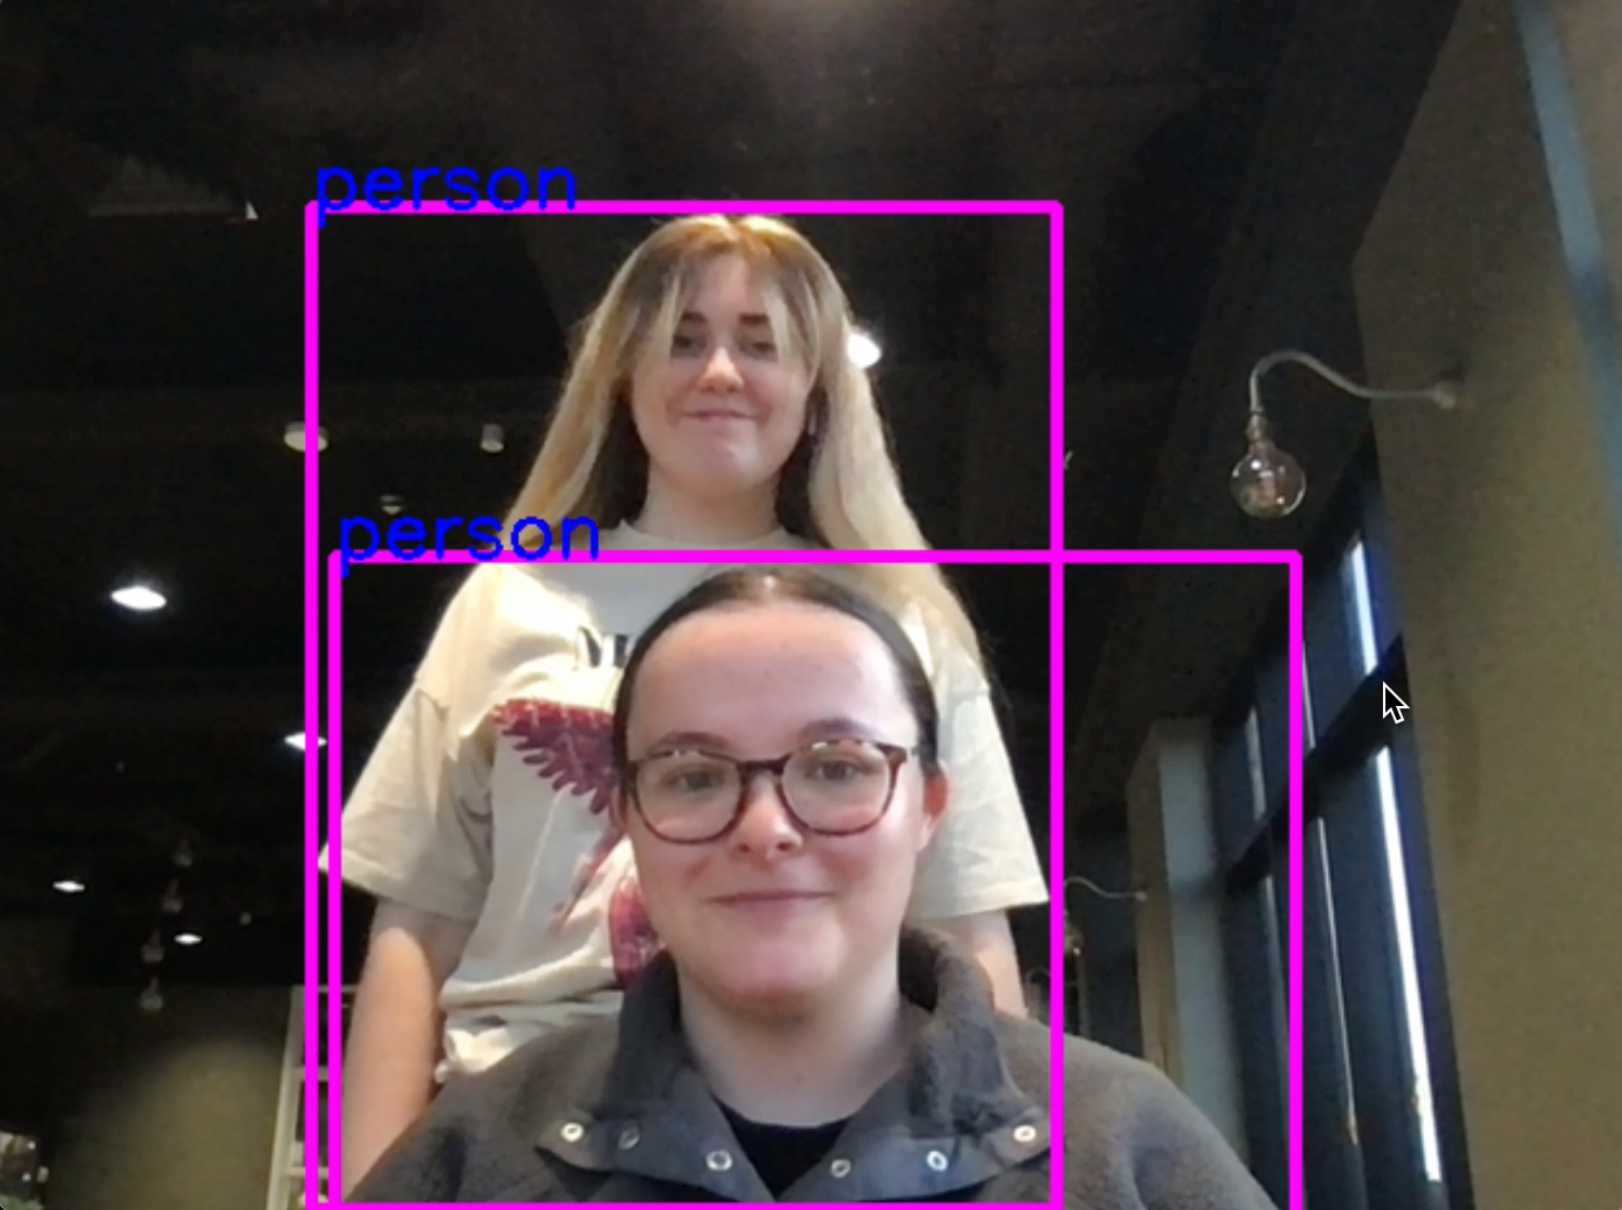
\includegraphics[width=.3\textwidth]{img/fig1-img1.png}\hfill
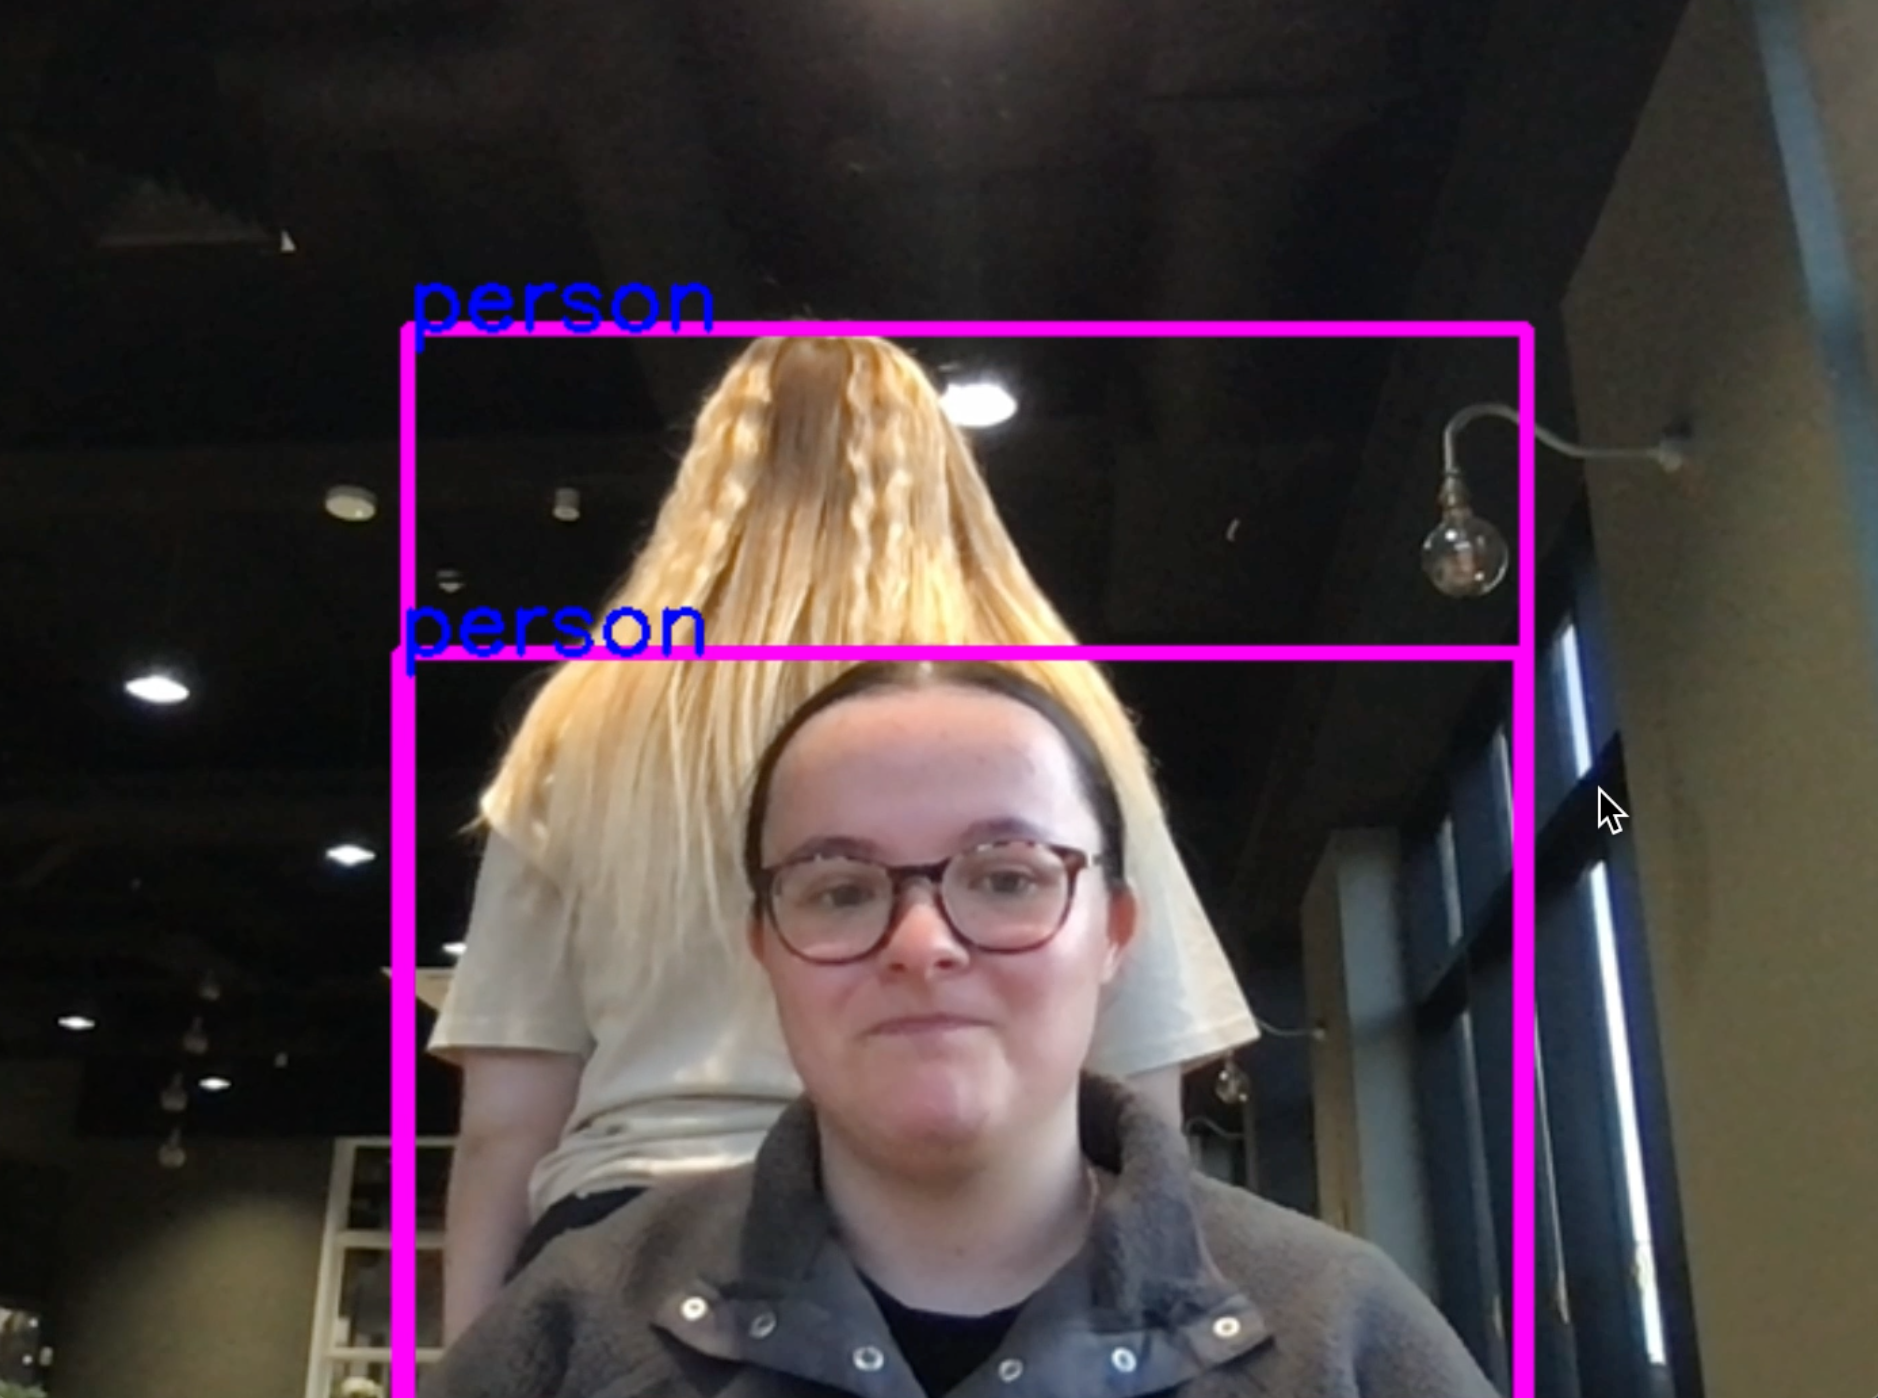
\includegraphics[width=.3\textwidth]{img/fig1-img2.png}\hfill
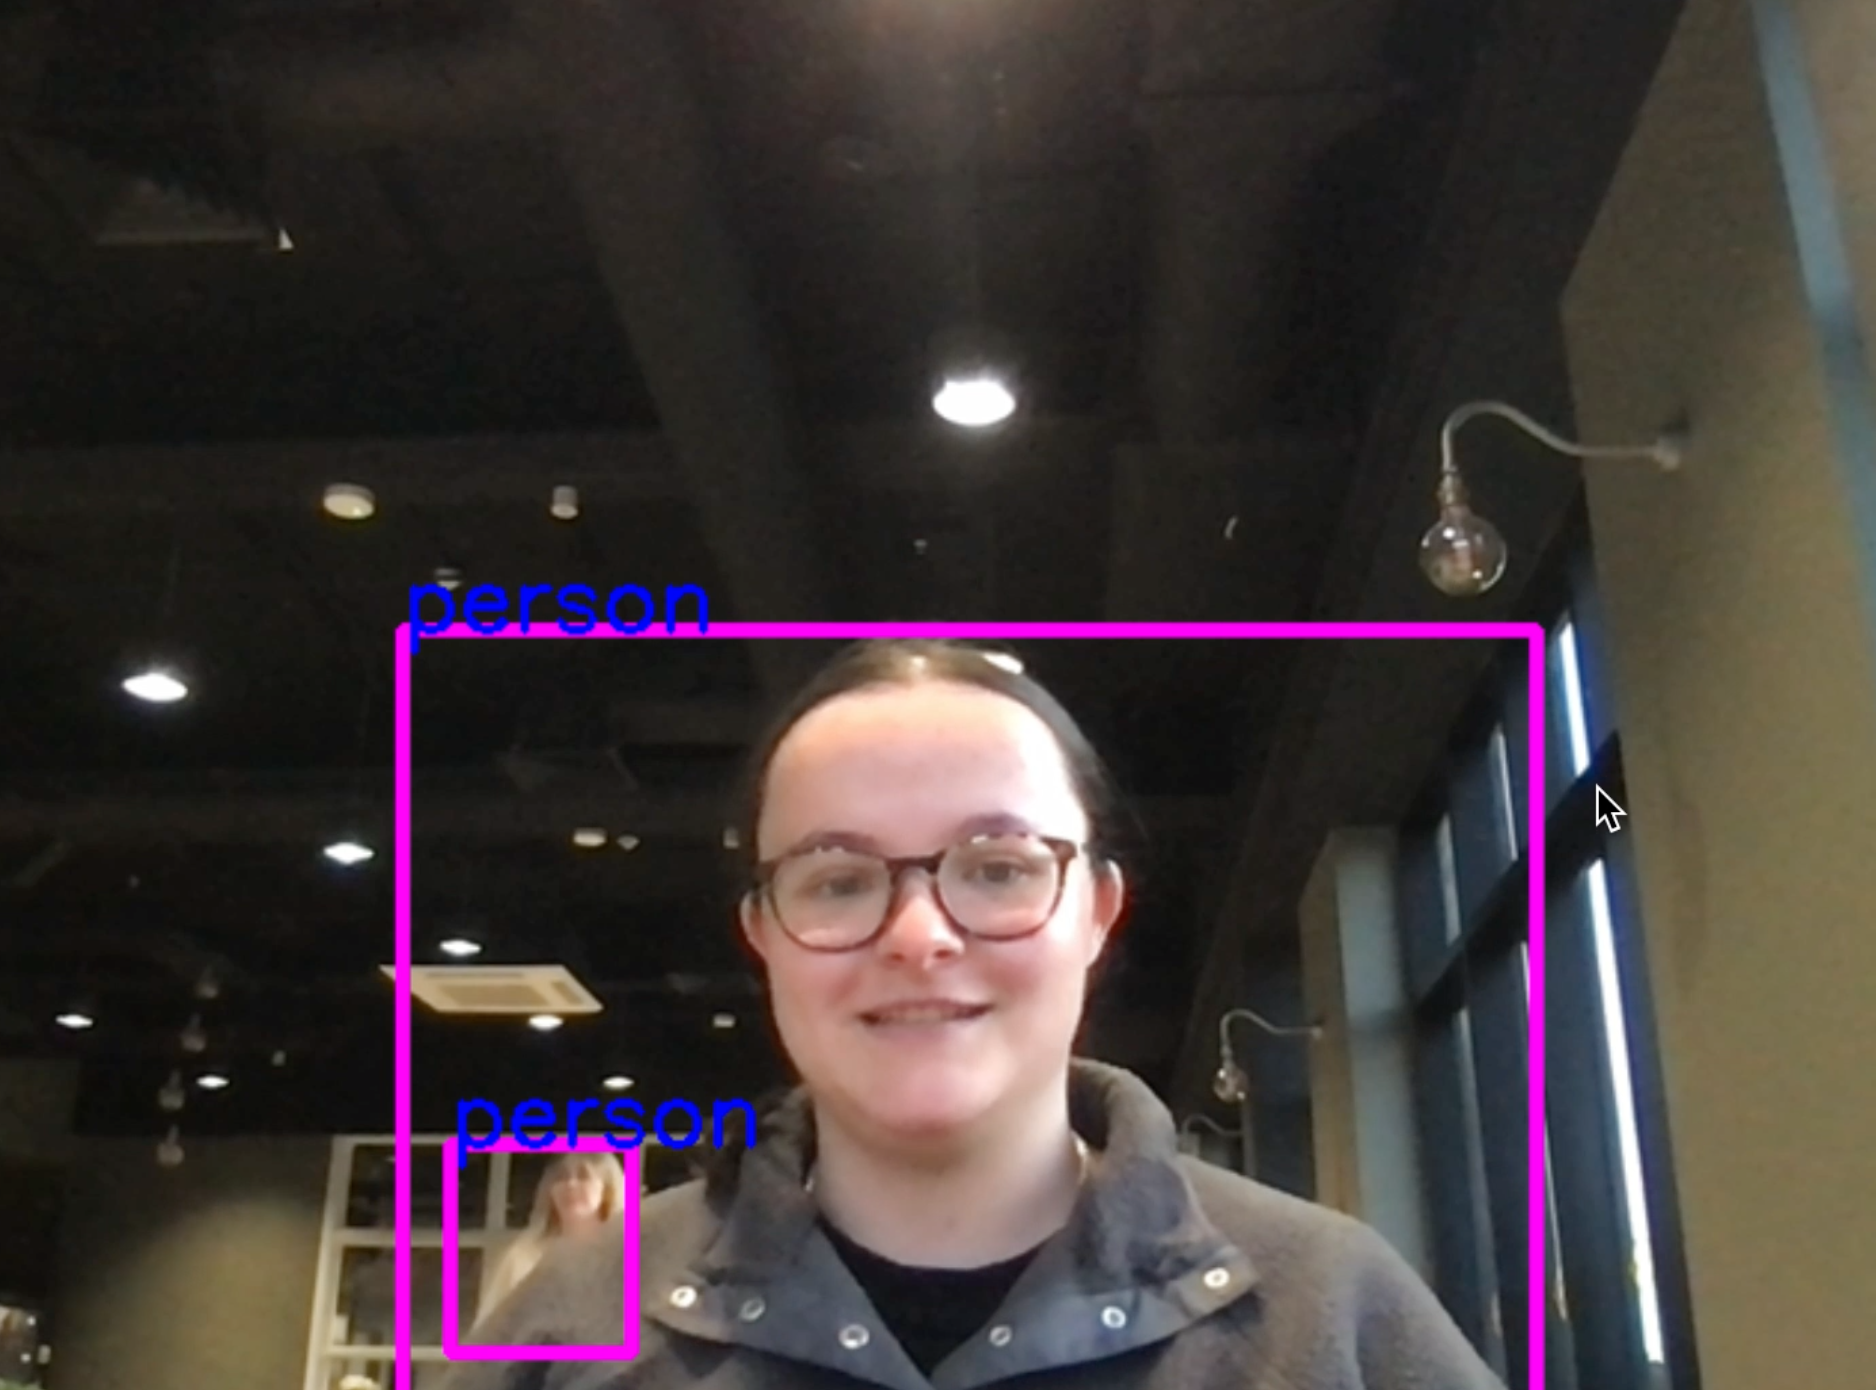
\includegraphics[width=.3\textwidth]{img/fig1-img3.png}\hfill

\caption{YOLO being used to detect more than one person in-front of the camera. The observer stands at different distances and angles to test the system.}
\label{fig:figure1}
\end{figure}

An experiment was carried out to test the limitations that using a front facing camera may have. The user stood 1 meter away from the camera, facing directly in the centre of the screen. They then slowly stepped to the left, decreasing the angle that they were to the screen, ensuring that they maintained a 1-meter distance at all times. As a result, the user was still visible and identifiable by the model until they were at a 35-degree angle to the screen. Figure~\ref{fig:figure2} shows the user where they could first not be identified.
\begin{figure}[ht]
  \centering
  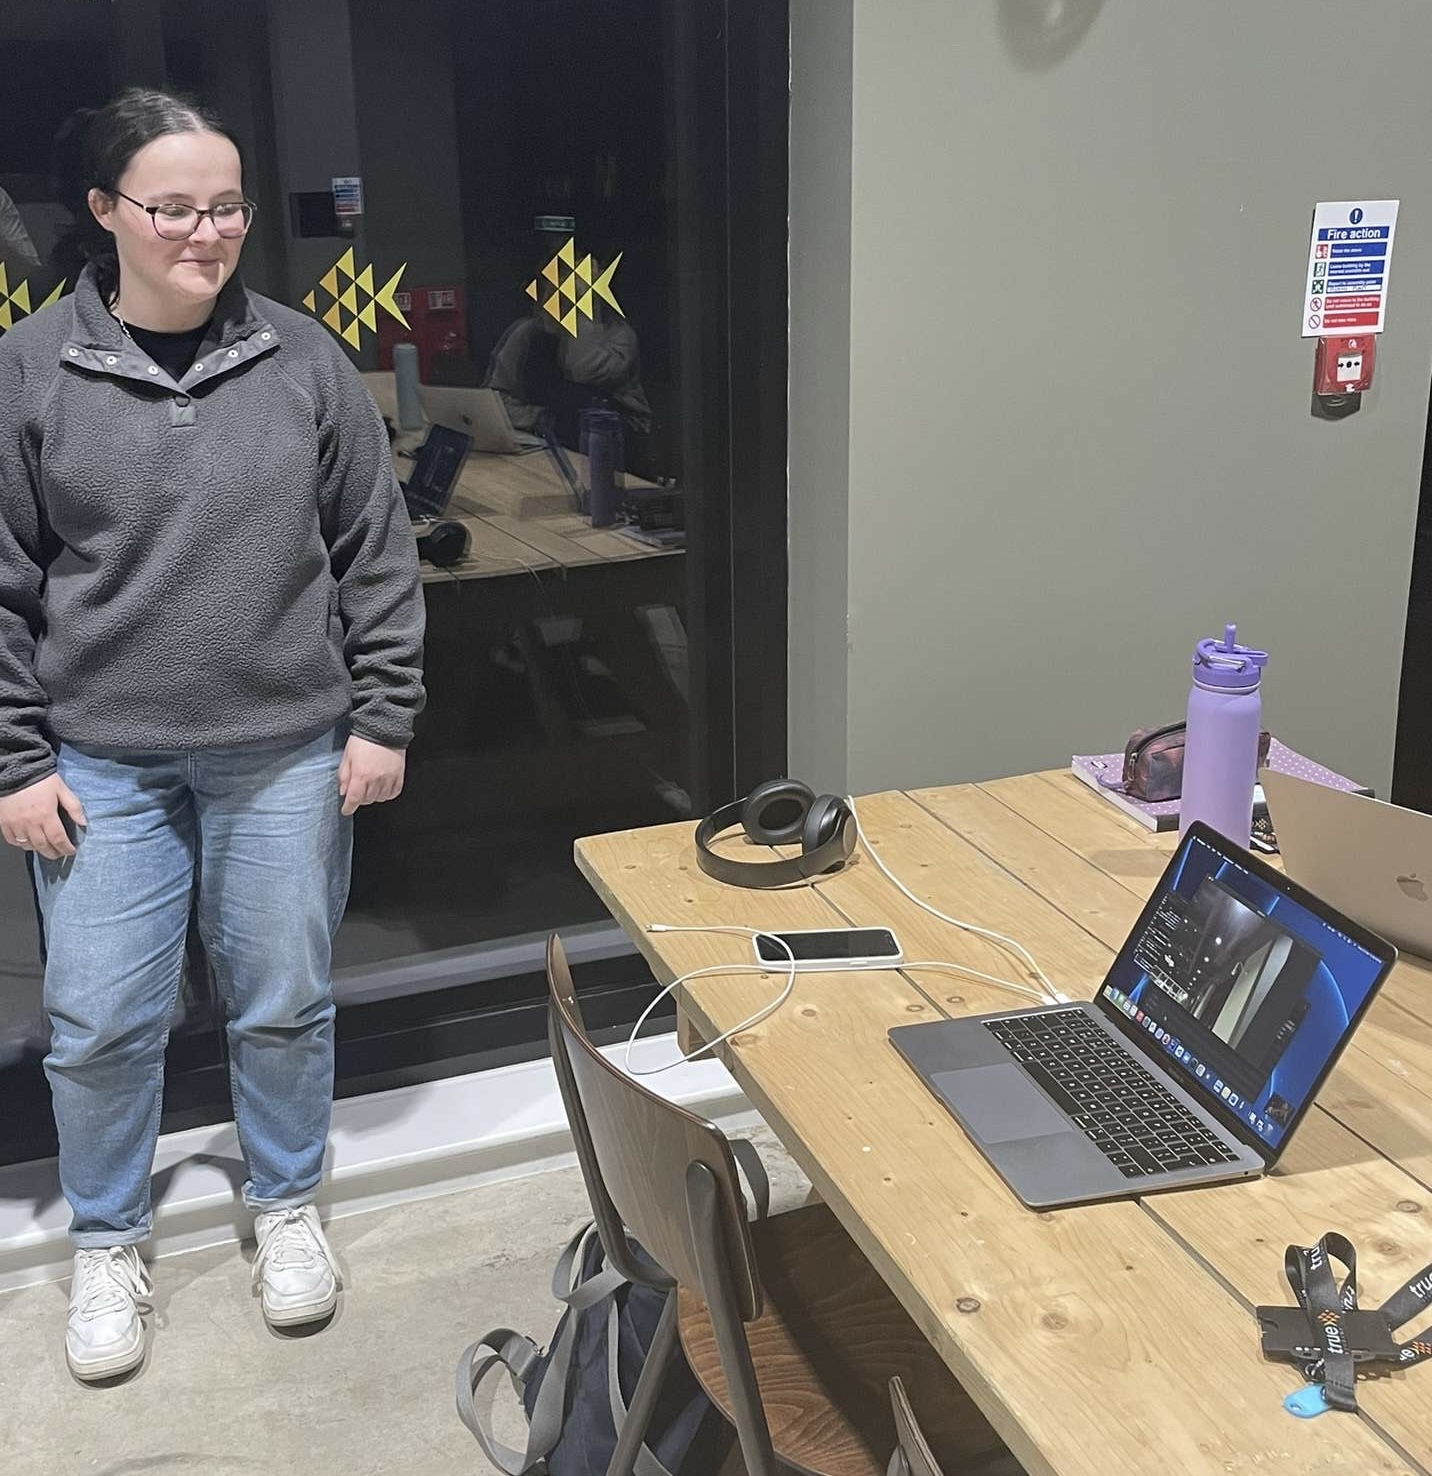
\includegraphics[width=70mm]{img/not_seen.jpg}
  \caption{The angle at which the YOLO model could no longer identify the user. }
  \label{fig:figure2}
\end{figure}

The experiment highlighted the limitations that the YOLO algorithm and camera may have. The user reported that they could still see what was on the screen meaning shoulder surfing could still take place. 
User studies will be carried out during the project to identify if it would be more beneficial to use a fish-eye camera which has a wider-angle view. It will be recorded if the user finds using an external device more cumbersome and if it benefits the results.


\section{Planning of the Project}
\label{sec:plan}
\subsection{Methodology}
The project will have a number of deliverables and aims which need to be met. An agile approach will be taken to ensure that all work is completed on time. The methodology will be slightly altered as this is a solo project and the final product will not be deployed. The project will be split into approximately three week sprints, allowing for continuos feedback and improvements. Whilst there will not be the typical sprint meeting normally used for teams, sprints will allow for the work to be broken up into more manageable sections. At the beginning of each sprint, key milestones that need to be met will be highlighted.  

Due to the technical aspects of the project, the software development life cycle (SDLC) should also be adhered to. Planning has started in this document and will continue up until the first prototype is created. Full research should be completed to ensure ideas are backed up and accurate. After prototypes have been created, the analysis stage can take place. User studies will be a way to understand the strengths and weaknesses of the product. More realistic prototypes can then be created allowing for the design stage to be met. As this project will not be deployed, the last stages in the SDLC will be changed. Heuristic evaluations can take place leading to improvements being made, tests should happen throughout the project to ensure the users needs are always being met.

\subsection{Gantt Chart}
A Gantt chart (Figure \ref{fig:figure3}) had been produced to allocate time to each task throughout the project. This ranges from the 30th September to 6th May when the project is due. Holidays have been considered and weekends have not been included. The agile approach allows for more than one sprint cycle so the dates may need to be updated after first evaluation. Some tasks overlap due to the nature of the project including the document writing and Gregynog presentation planning.

\begin{figure}[!htb]
  \centering
  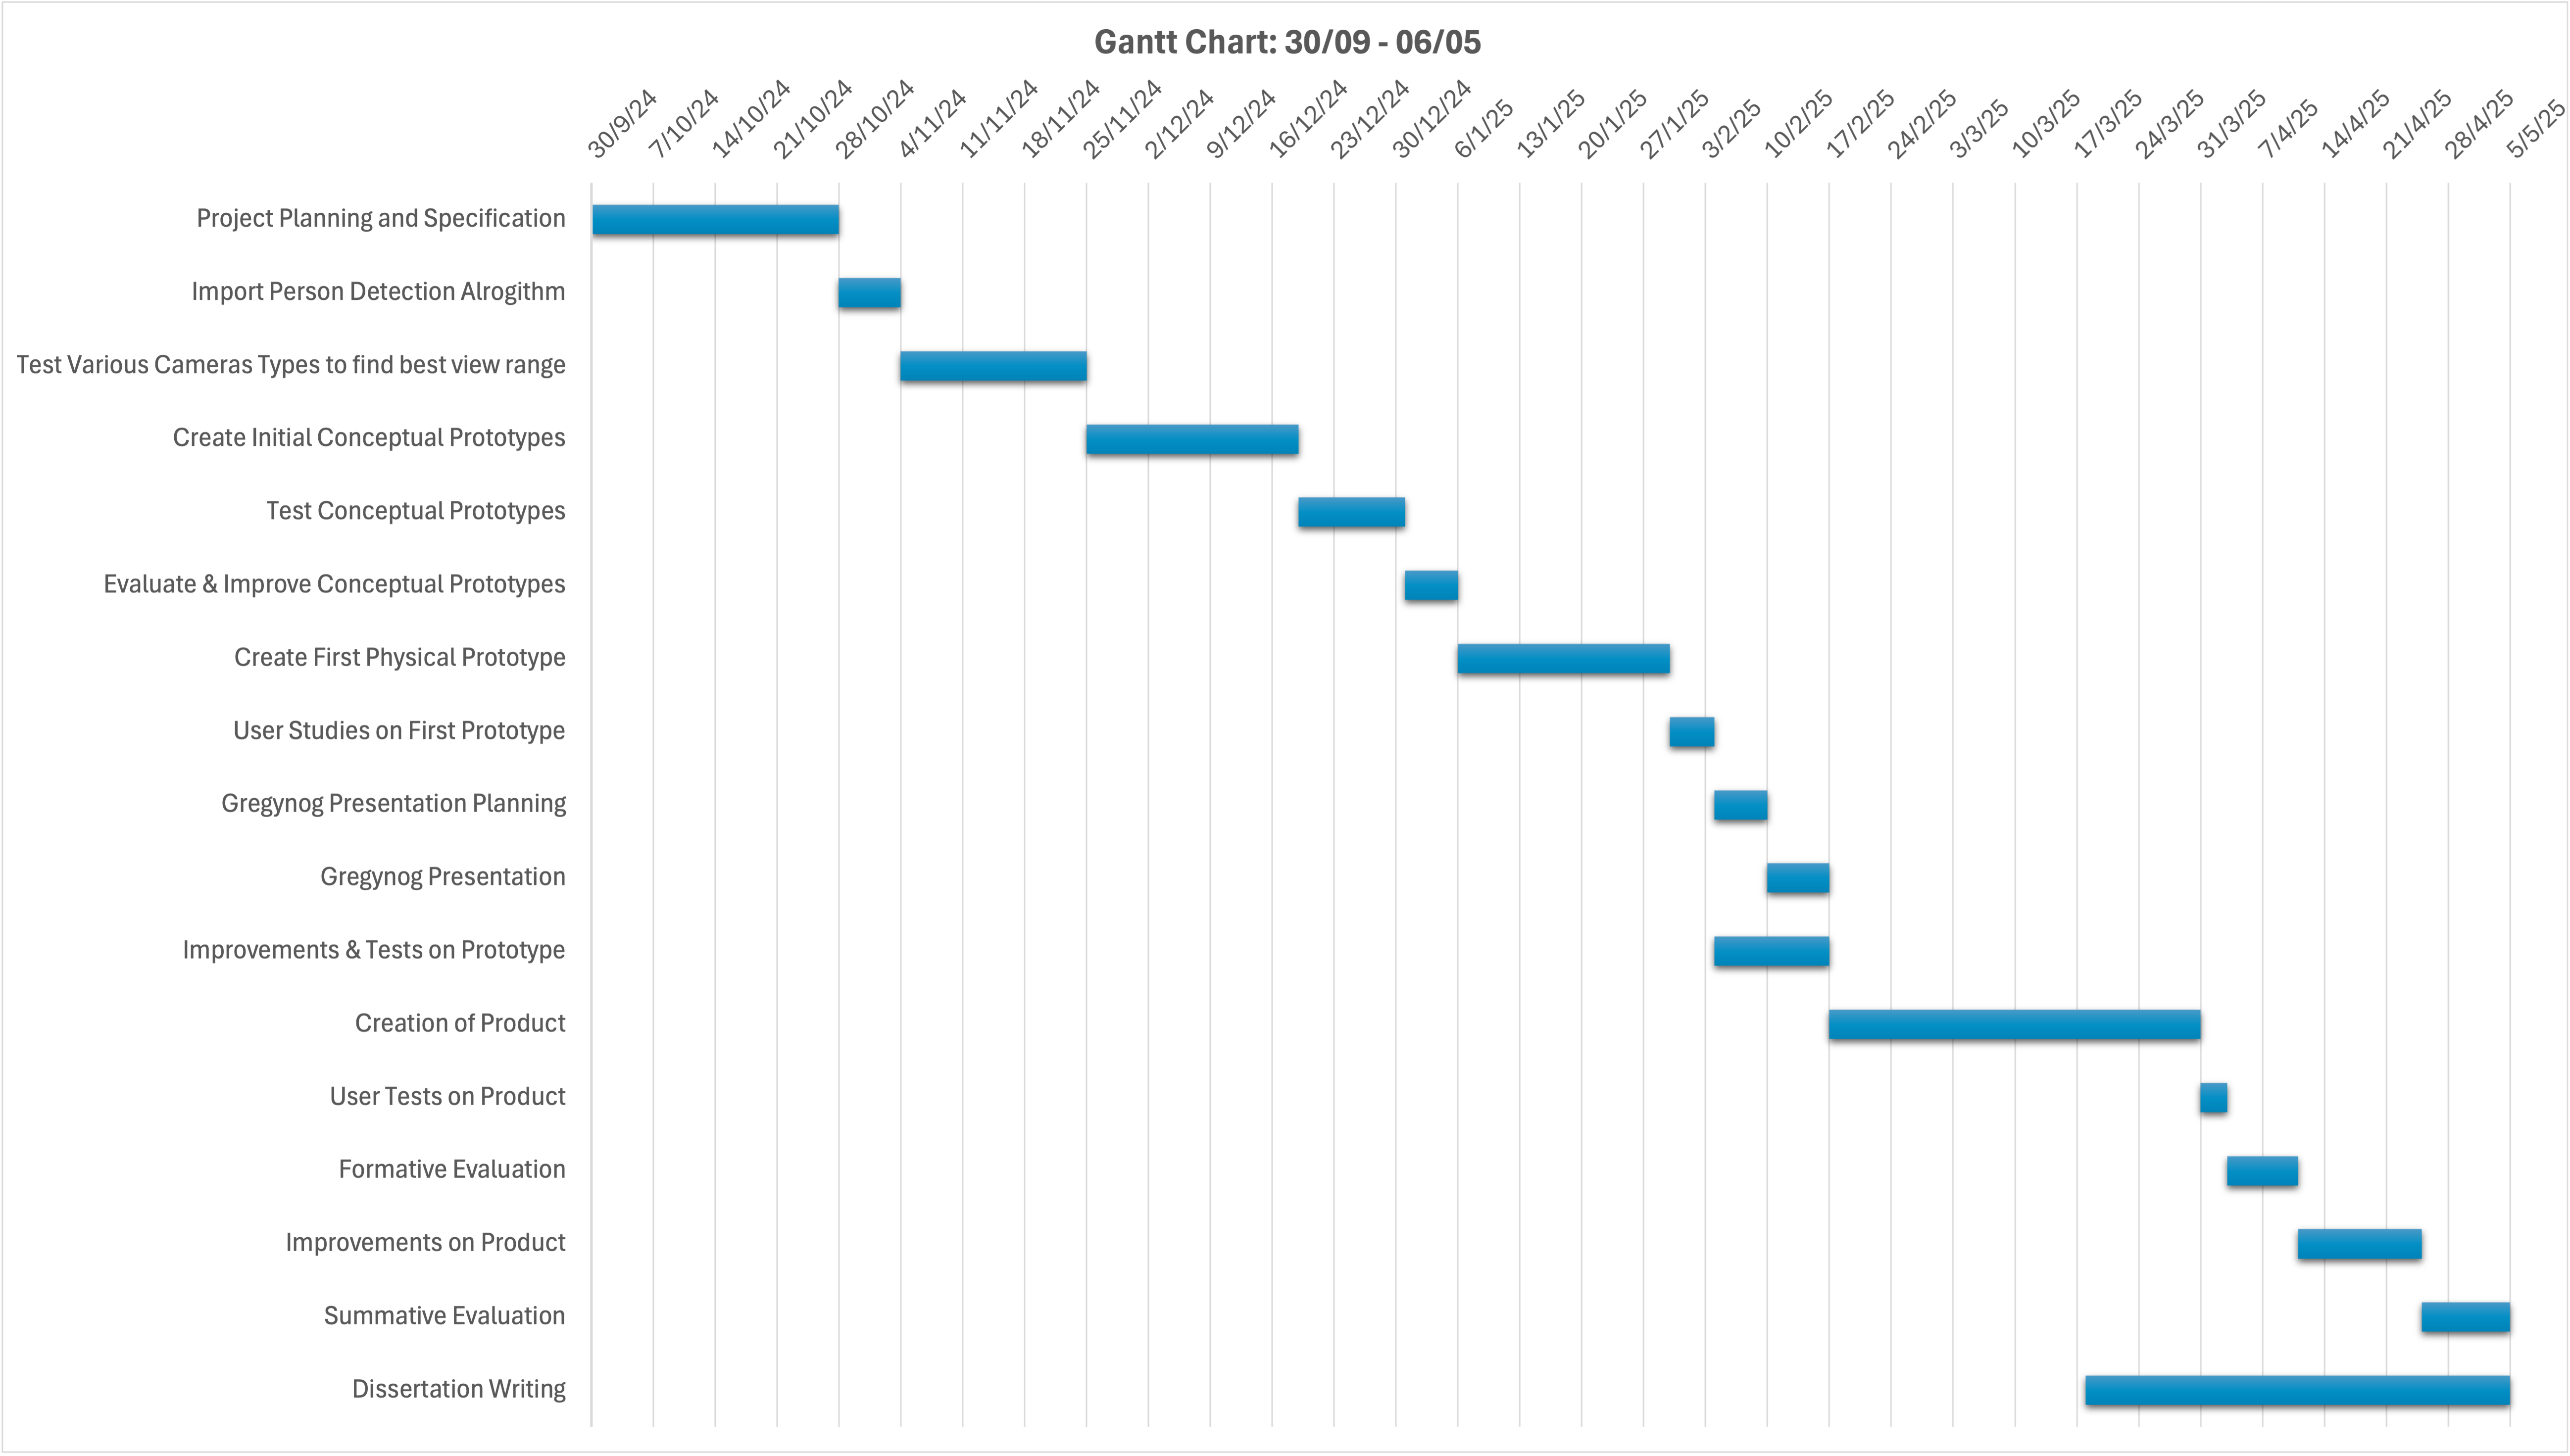
\includegraphics[width=\linewidth]{Picture 1.png}
  \caption{A Gantt Chart with key deliverables for the project. }
  \label{fig:figure3}
\end{figure}

Key milestones in the project are as follows:
\begin{itemize}
\item \emph{Project Specification and Planning Document}.
\item \emph{Gregynog Presentation}.
\item \emph{Initial Conceptual Prototypes}. Low-fidelity prototypes (e.g. storyboards, Wizard of Oz) will be created so that exploration into details can take place.
\item \emph{Testing Conceptual Prototypes}. Experiments of the low-fidelity prototypes will take place to highlight any major modifications needed.
\item \emph{Initial Physical Prototype}. A version of software will be created, highly likely that bugs will still occur. 
\item \emph{User Studies}. The high-fidelity prototype will be used in a user study to find weaknesses in the product.
\item \emph{Real Product Creation}. Software will be produced with an appropriate UI where bugs are not present.
\item \emph{Further User Studies and Analysis}. The UI will be tested and users thoughts will be welcome. Changes after feedback will also take place at this time.
\item \emph{Formative Evaluation}. This evaluation will take place during design to ensure the product is meeting the users needs.
\item \emph{Summative Evaluation}. This will access the final product. The projects aims and objectives will be used to evaluate the success of the project.
\item \emph{Dissertation Document Writing}.
\end{itemize}



\section{Risk Analysis}
\label{sec:risk}

Tables \ref{tab:risks1} and \ref{tab:risks2} identify and rank the potential risks that may occur when carrying out the project. The potential impact is measured on a Likert scale where 1 is insignificant and 5 is very significant. The likelihood is also measured on a Likert scale where 1 is rare and 5 is very likely. All of the identified risks have been scored using the following formula:
\[
  Risk Score = Likelihood \times Potential Impact
\]
The scores can then be compared, the highest score will be 1 and will continue until the lowest score is found. Ranking allows us to understand which mitigation measures should be taken into account more.

\newgeometry{left=5mm, right=5mm}
\begin{table}[]
\centering
\begin{tabular}{|l|l|l|l|l|l|}
\hline
\textbf{Identified Risks} &
  \textbf{\begin{tabular}[c]{@{}l@{}}Like-\\ lihood\end{tabular}} &
  \textbf{\begin{tabular}[c]{@{}l@{}}Potential \\ Impact\end{tabular}} &
  \textbf{Risk Mitigation} &
  \textbf{\begin{tabular}[c]{@{}l@{}}Risk \\ Score\end{tabular}} &
  \textbf{\begin{tabular}[c]{@{}l@{}}Risk \\ Rank\end{tabular}} \\ \hline
\begin{tabular}[c]{@{}l@{}}Not able to find any users for \\ user studies.\end{tabular} &
  3 &
  4 &
  \begin{tabular}[c]{@{}l@{}}Users will be found in advance to the\\ start of user studies. Incentives can \\ be put in place to help increase the\\ chance of gaining participants.\end{tabular} &
  12 &
  2 \\ \hline
\begin{tabular}[c]{@{}l@{}}The software incorrectly \\ identifies a person. For \\ example, a person is not \\ detected at all or another\\ object is identified as a person.\end{tabular} &
  3 &
  3 &
  \begin{tabular}[c]{@{}l@{}}One of the first milestones is to \\ import the object detection algorithm,\\ once this is completed it should be \\ stress tested to ensure incorrect \\ identification does not take place.\end{tabular} &
  9 &
  4 \\ \hline
\begin{tabular}[c]{@{}l@{}}The software does not identify \\ a shoulder surfing attack.\end{tabular} &
  4 &
  5 &
  \begin{tabular}[c]{@{}l@{}}This will be one of the main focusses\\ of the project, user studies will be \\ carried out to test this risk. If an \\ attack is not identified, the screen \\ brightness will not change and the \\ user will not be notified. Initial \\ prototypes should also investigate \\ this threat and ways to reduce it.\end{tabular} &
  20 &
  1 \\ \hline
User data privacy concerns. &
  2 &
  4 &
  \begin{tabular}[c]{@{}l@{}}The software will access the devices\\ camera and detect threats from this.\\ Users may raise the concern that they\\ are constantly being filmed and \\ 'watched'. To eliminate this, the data \\ will not be saved or stored so will\\ not be accessible by anyone. The \\ user will always have the option to \\ stop the software meaning the\\ camera will no longer be accessed.\end{tabular} &
  8 &
  5 \\ \hline
  \begin{tabular}[c]{@{}l@{}}Hardware incompatibility may \\ take place meaning the \\ software cannot be run.\end{tabular} &
  1 &
  5 &
  \begin{tabular}[c]{@{}l@{}}The software needs to make a \\ connection with the devices \\ camera. When there is not a \\ built-in camera, a plug-in \\ external camera will need to be\\ used. A test during the first agile\\ sprint will check that the software \\ works on a range of devices and OS's.\end{tabular} &
  5 &
  6 \\ \hline
\end{tabular}
\caption{Risk analysis for project.}
  \label{tab:risks1}
\end{table}
\restoregeometry

\newgeometry{left=5mm, right=5mm}
\begin{table}[]
\centering
\begin{tabular}{|l|l|l|l|l|l|}
\hline
\textbf{Identified Risks} &
  \textbf{\begin{tabular}[c]{@{}l@{}}Like-\\ lihood\end{tabular}} &
  \textbf{\begin{tabular}[c]{@{}l@{}}Potential \\ Impact\end{tabular}} &
  \textbf{Risk Mitigation} &
  \textbf{\begin{tabular}[c]{@{}l@{}}Risk \\ Score\end{tabular}} &
  \textbf{\begin{tabular}[c]{@{}l@{}}Risk \\ Rank\end{tabular}} \\ \hline
\begin{tabular}[c]{@{}l@{}}The user's environment may \\ reduce the success rate of \\ the shoulder surfer detector.\end{tabular} &
  3 &
  4 &
  \begin{tabular}[c]{@{}l@{}}When the user is in a busier \\ environment,  it is likely that more\\ people will pass by the camera \\ resulting in more threats being \\ accessed. Room lighting and camera\\ angles will also have an impact on \\ the detector.  All of these factors \\ will have to be tested during user\\ studies and mitigated before the \\ final development.\end{tabular} &
  12 &
  2 \\ \hline
\begin{tabular}[c]{@{}l@{}}In public spaces, onlookers \\ may not give direct permission\\  to be analysed by the detector.\end{tabular} &
  5 &
  2 &
  \begin{tabular}[c]{@{}l@{}}The algorithm will detect anybody\\ that is in camera view meaning \\ those in the background may be \\ recorded. Legislations will have to be \\ checked to ensure that no laws are\\ breached before testing can take \\ place. All users will be told how\\ the technology works before taking \\ part and will be warned that a \\ camera will be used.\end{tabular} &
  10 &
  3 \\ \hline
\begin{tabular}[c]{@{}l@{}}Project interruptions causing\\ progress to fall behind the\\ set out plan.\end{tabular} &
  4 &
  1 &
  \begin{tabular}[c]{@{}l@{}}Other project deadlines and risks \\ may cause the project to fall off\\ plan. A two week buffer has been \\ added to the Gantt chart during \\ December to help reduce this. \\ The agile sprints should raise any\\  fallbacks before they become\\  a major issue and should be \\ sorted so the project is back on \\ plan as soon as possible.\end{tabular} &
  4 &
  7 \\ \hline
\end{tabular}
\caption{Cont: Risk analysis for project.}
  \label{tab:risks2}
\end{table}
\restoregeometry

\section{Conclusions}
\label{sec:conclusion}

A review of past literature has been completed, highlighting the gaps for future work which this project will start to explore. There is a need for user-centered design within shoulder surfing detection so a object detection algorithm will be imported. This algorithm has been identified and researched to ensure it will meet the needs of the project.

A project methodology has been evaluated to ensure the project stays on track, and risks have been identified with mitigation techniques. A Gantt chart will be followed which includes key milestones for the software product. Having project aims and objectives will allow for extensive summative evaluation at the end of the project.

% Prints the Reference section
\printbibliography

% Appendices are used to provide bulk information that does not fit
% into the main text. Common content is program code and data
% sets. You may want to discuss key elements in the main text, but
% provide the rest in an appendix for completeness.
\clearpage\appendix

\end{document}
